
\begin{figure}
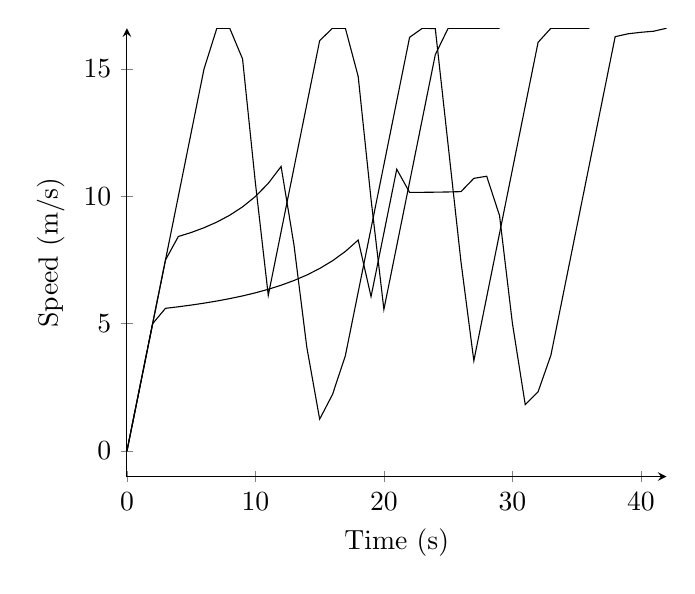
\begin{tikzpicture}
\begin{axis}[
legend style={anchor=west},
axis x line=bottom,
axis y line=left,
ymin=-1,
xlabel=Time (s),
ylabel=Speed (m/s),
]
\addplot[] coordinates {
(0, 0.0)
(1, 2.5)
(2, 5.0)
(3, 7.5)
(4, 8.42289323598)
(5, 8.58083512054)
(6, 8.76737736151)
(7, 8.98992901986)
(8, 9.25848631303)
(9, 9.58680755238)
(10, 9.99426633665)
(11, 10.5088733966)
(12, 11.1723976924)
(13, 8.09596358988)
(14, 4.07693536988)
(15, 1.2540610702)
(16, 2.22025967764)
(17, 3.74325259661)
(18, 6.24325259661)
(19, 8.74325259661)
(20, 11.2432525966)
(21, 13.7432525966)
(22, 16.2432525966)
(23, 16.6)
(24, 16.5838198363)
(25, 12.0091906029)
(26, 7.42462881929)
(27, 3.54594747022)
(28, 6.04594747022)
(29, 8.54594747022)
(30, 11.0459474702)
(31, 13.5459474702)
(32, 16.0459474702)
(33, 16.6)
(34, 16.6)
(35, 16.6)
(36, 16.6)
};
\addplot[] coordinates {
(0, 0.0)
(1, 2.5)
(2, 5.0)
(3, 7.5)
(4, 10.0)
(5, 12.5)
(6, 15.0)
(7, 16.6)
(8, 16.6)
(9, 15.3934569437)
(10, 10.5214562517)
(11, 6.11202054391)
(12, 8.61202054391)
(13, 11.1120205439)
(14, 13.6120205439)
(15, 16.1120205439)
(16, 16.6)
(17, 16.6)
(18, 14.7050672306)
(19, 9.88203394578)
(20, 5.56090804849)
(21, 8.06090804849)
(22, 10.5609080485)
(23, 13.0609080485)
(24, 15.5609080485)
(25, 16.6)
(26, 16.6)
(27, 16.6)
(28, 16.6)
(29, 16.6)
};
\addplot[] coordinates {
(0, 0.0)
(1, 2.5)
(2, 5.0)
(3, 5.60387224087)
(4, 5.66434851162)
(5, 5.7315179936)
(6, 5.80641440752)
(7, 5.89028076279)
(8, 5.98462277049)
(9, 6.09127898453)
(10, 6.21251397629)
(11, 6.35114366696)
(12, 6.51070623913)
(13, 6.69569872745)
(14, 6.91190998506)
(15, 7.16689793254)
(16, 7.47068766403)
(17, 7.83681611636)
(18, 8.28393591486)
(19, 6.06350899493)
(20, 8.56350899493)
(21, 11.0635089949)
(22, 10.1537141517)
(23, 10.1577868131)
(24, 10.1635184918)
(25, 10.1719557222)
(26, 10.1851299763)
(27, 10.7065958809)
(28, 10.789188156)
(29, 9.24555957001)
(30, 5.02181345163)
(31, 1.82423225263)
(32, 2.32633312518)
(33, 3.76790634463)
(34, 6.26790634463)
(35, 8.76790634463)
(36, 11.2679063446)
(37, 13.7679063446)
(38, 16.2679063446)
(39, 16.3812995377)
(40, 16.4398523735)
(41, 16.4826320982)
(42, 16.6)
};

\end{axis}
\end{tikzpicture}
\label{tik:speed:100:45}
\caption{100 percent diving with GSC on route $45$}
\end{figure}
